% Opus Operandi -- technical document, More than a Hack 2027, phase 1.
% Build:  cd docs/latex && tectonic Opus_Operandi.tex      (or: pdflatex Opus_Operandi.tex, twice)
% Figures are read from ../figures/ (redraw them with: python scripts/make_figures.py).
\documentclass[10pt,a4paper]{article}
\usepackage[a4paper,margin=2.0cm,top=1.8cm,bottom=2.0cm]{geometry}
\usepackage[T1]{fontenc}
\usepackage[utf8]{inputenc}
\usepackage{lmodern}
\usepackage{microtype}
\usepackage{amsmath,amssymb}
\usepackage{graphicx}
\usepackage{booktabs}
\usepackage{tabularx}
\usepackage{array}
\usepackage[table]{xcolor}
\usepackage{enumitem}
\usepackage{caption}
\usepackage{float}
\usepackage[most]{tcolorbox}
\usepackage{fancyhdr}
\usepackage[hidelinks]{hyperref}
\usepackage{url}

\graphicspath{{../figures/}}
\definecolor{oblue}{HTML}{2A78D6}
\definecolor{oink}{HTML}{1F3A5F}
\definecolor{ogrey}{HTML}{52514E}
\definecolor{oboxbg}{HTML}{EEF5FD}
\hypersetup{colorlinks=true,linkcolor=oink,urlcolor=oink,citecolor=oink}
\captionsetup{font=small,labelfont=bf,labelsep=period}
\setlist{itemsep=1pt,topsep=3pt,leftmargin=*}
\newcolumntype{L}{>{\raggedright\arraybackslash}X}
\renewcommand{\arraystretch}{1.15}
\pagestyle{fancy}
\fancyhf{}
\renewcommand{\headrulewidth}{0pt}
\fancyfoot[L]{\footnotesize\color{ogrey}Opus Operandi --- More than a Hack 2027, phase 1: technical document}
\fancyfoot[R]{\footnotesize\color{ogrey}\thepage}
\newcommand{\code}[1]{\texttt{\small #1}}
\newcommand{\fig}[3][0.92]{\begin{figure}[H]\centering\includegraphics[width=#1\linewidth]{#2}\caption{#3}\end{figure}}

\begin{document}

\begin{center}
{\LARGE\bfseries\color{oink} Opus Operandi: possession that survives the missing ball}\\[4pt]
{\large More than a Hack 2027, phase 1 --- frame-level ball possession, FC Barcelona vs Athletic Club}\\[6pt]
Team \textit{Opus Operandi}\\
Alejandro Coves Bolaños, Jesús Sánchez Briñas, Lucas Borges de Castro, Lorena Almoguera Romero, Ismael Mohamed Mohamed\\[2pt]
Code: \url{https://github.com/Opus-Operandi-FC-Barcelona/mtah2027-possession-engine}\\
{\small Other-match benchmarks: \code{mtah2027-external-benchmarks}. Lab notebook with every experiment: \code{docs/TECHNICAL\_REPORT.md}.}
\end{center}

\begin{tcolorbox}[colback=oboxbg,colframe=oblue,boxrule=0.8pt,arc=2pt,left=8pt,right=8pt,top=4pt,bottom=4pt,
  title={\bfseries At a glance},coltitle=oink,colbacktitle=oboxbg,toptitle=2pt,bottomtitle=0pt]
\begin{itemize}
\item A deterministic engine labels all \textbf{199,319 frames}. Football logic does the segmentation: a possession changes hands only at a touch, and a restart starts where the tracking shows the ball leaving rest. Learned models supply the evidence.
\item Two calibrated LightGBM \textbf{specialists} (ball visible / ball hidden) and a \textbf{non-causal TCN} ($\pm$20\,s of context) are trained only on \textbf{other matches}: 7 Bundesliga (IDSSE/DFL) and World Cup 2022 (PFF). Labels come from algorithms, never from hand annotation.
\item Key finding: in BAR-ATH \textbf{the ball goes missing mostly while it is dead}. A label-free estimator puts this at $\geq$\,80\,\% of hidden-ball frames, against 41\,\% if gaps were random. Training in that estimated world was our largest data-side gain.
\item \textbf{31 ideas} were built and measured under one preregistered rule ($\geq$\,+0.010 spellF1, no seed below $-0.003$). \textbf{5 were adopted}; the other 26 stay in the code, off by configuration.
\item External validation (official metric): spellF1 \textbf{0.739} on IDSSE leave-one-match-out and \textbf{0.680} (macroF1 0.902) on \textbf{8 PFF matches never used for anything}. Public window: spellF1 \textbf{0.700} (macroF1 0.898), against 0.424 for the best baseline. The CSV is \textbf{byte-for-byte reproducible}, and the SHA256 is checked on Windows and Linux CI.
\end{itemize}
\end{tcolorbox}

\section{The task, and why it is hard}
Each frame of the tactical video gets \code{H} (Barcelona in possession), \code{A} (Athletic in possession), \code{D} (ball dead) or \code{X} (not graded). The ranking metric treats every possession, a maximal run of \code{H} or \code{A}, as one object. Predicted and true possessions of the same team are matched one-to-one by temporal IoU, and F1 is averaged over five thresholds:
\begin{equation}
\mathrm{spellF1} = \frac{1}{5}\sum_{\theta\in\{0.3,\dots,0.7\}} \frac{2\,TP_\theta}{2\,TP_\theta+FP_\theta+FN_\theta},
\end{equation}
with macroF1 over \code{H}, \code{A}, \code{D} as the tie-break. Three consequences drove every design choice:
\begin{itemize}
\item \textbf{Segmentation beats frame accuracy.} A one-second flicker invents a possession and can split a true one. A per-frame classifier with 90\,\% accuracy can still score badly.
\item \textbf{A \code{D} splits a possession}, so finding stoppages matters as much as the team call.
\item \textbf{Boundaries must be within a few frames.} A one-frame offset is free; a one-second offset costs about 0.35.
\end{itemize}
And the data fights back. The tracking is automatic and uncorrected: slots are tracklets, not players. The ball is untracked on about 41\,\% of graded frames, in long blocks. On average 20.5 players are tracked, and 14.2\,\% of frames have fewer than 20. The public window, with the ball present most of the time and only 17 possessions, is far easier than the rest of the match. One possession moves its spellF1 by about 0.06, so we never used it to choose anything.
\fig{ball_presence.png}{Share of frames with a tracked ball (top) and tracked players (bottom), 30\,s means over the whole video. Grey: graded halves. Green: the public window.}

\section{Results}
\subsection{External validation: the numbers we trust}
Every decision was taken on other matches, scored with the official \code{possession\_metrics.py}:
\begin{itemize}
\item \textbf{B$'$(33)}, primary criterion: the 7 IDSSE matches, leave-one-match-out (the held-out match is an unlabelled target), degraded with the calibrated degrader in the estimated ``gaps over dead ball'' world, evaluation seeds 0--2.
\item \textbf{B$'$(1)}, guard: the same matches with gaps placed at random.
\item \textbf{A}, guard: 20 PFF matches with real occlusions (the ball missing in about a third of the frames).
\item \textbf{Unseen PFF}, independent check: 8 further PFF matches (\code{pff\_3852}--\code{pff\_3859}) that never entered training or selection.
\end{itemize}
\fig{validation_ladder.png}{Each adopted step, on the primary criterion (left) and on the 8 never-used PFF matches (right). The ordering is identical on both, so the gains are not an artefact of the tuning matches.}

\begin{table}[H]\centering\footnotesize\setlength{\tabcolsep}{4pt}
\begin{tabular}{lcccc}
\toprule
route & IDSSE B$'$(33) & IDSSE B$'$(1) & PFF A (20) & PFF unseen (8)\\
\midrule
Heuristic route (no learning) & -- & -- & -- & 0.295\\
Specialists A/B (pre-\#72) & 0.669 & 0.602 & 0.526 & 0.526\\
+ sequence TCN on hidden-ball frames (\#72) & 0.682 & 0.641 & 0.600 & 0.616\\
\textbf{+ TCN on visible frames too (\#73, submitted)} & \textbf{0.739} & \textbf{0.684} & \textbf{0.660} & \textbf{0.680}\\
\bottomrule
\end{tabular}
\caption{spellF1 with the official metric on other matches. On the unseen PFF matches the submitted route reaches macroF1 0.902.}
\end{table}

\begin{figure}[H]\centering
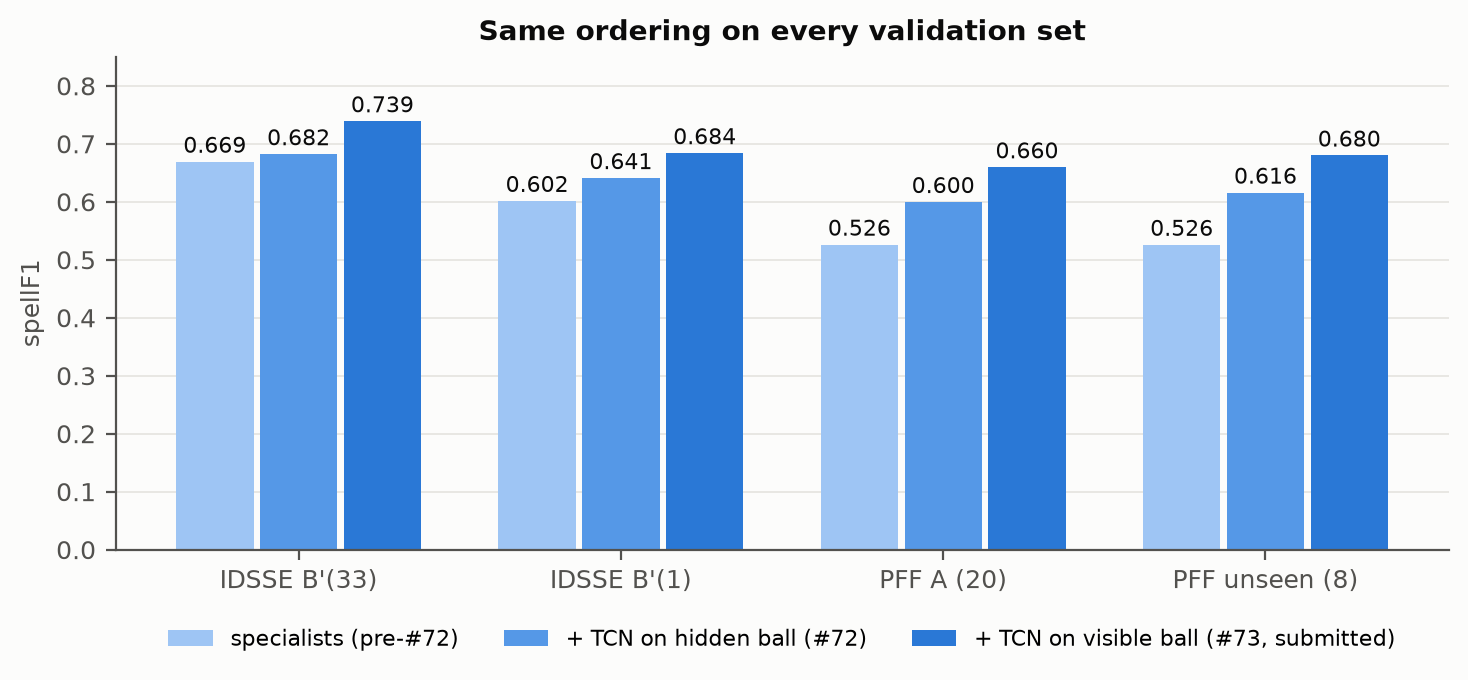
\includegraphics[width=0.49\linewidth]{validation_sets.png}\hfill
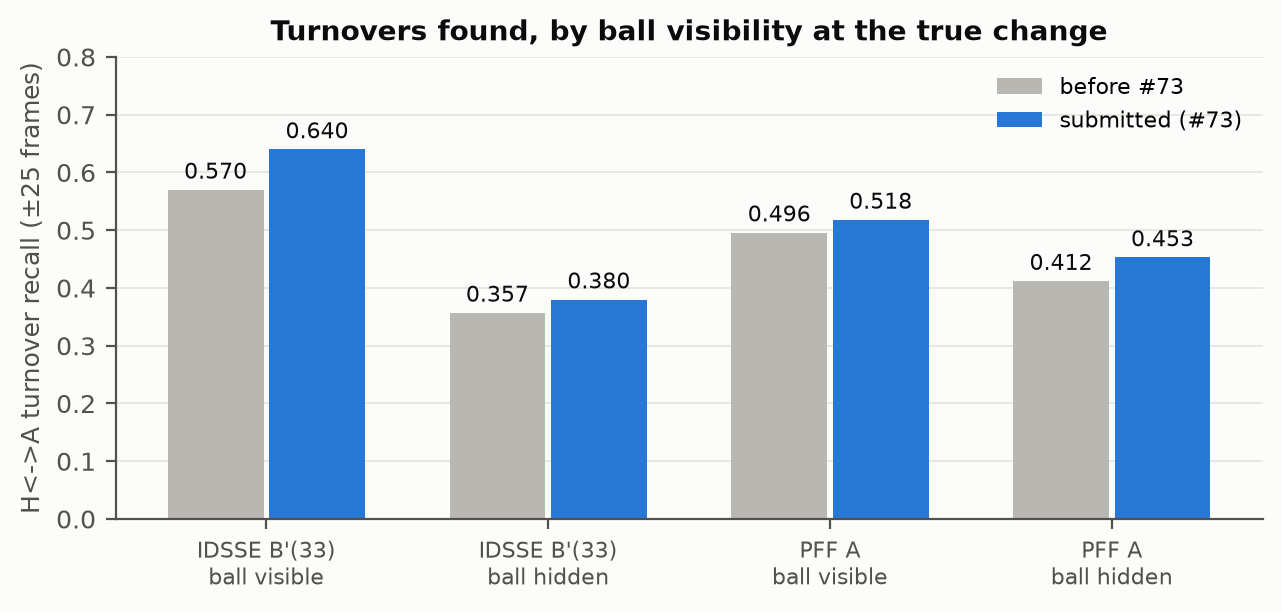
\includegraphics[width=0.49\linewidth]{turnover_recall.png}
\caption{Left: the three routes on the four validation sets. Right: H$\leftrightarrow$A turnovers matched within $\pm$25 frames. On IDSSE, recall rises from 0.570 to 0.640 with the ball visible and from 0.357 to 0.380 with it hidden, while spurious turnovers drop from 2742 to 2477.}
\end{figure}

\subsection{Public window (official scorer, pipeline check only)}
\begin{table}[H]\centering\small
\begin{tabular}{lccccc}
\toprule
submission & spellF1 & macroF1 & possessions & mean duration & latency\\
\midrule
\textbf{Opus Operandi} & \textbf{0.7000} & \textbf{0.8978} & 15 & 16.7\,s & +2.8 frames\\
baseline\_smooth125 & 0.4242 & 0.5812 & 16 & 18.5\,s & \\
baseline\_smooth50 & 0.3256 & 0.6207 & 26 & 10.8\,s & \\
baseline\_smooth25 & 0.2868 & 0.6200 & 36 & 7.6\,s & \\
baseline\_raw & 0.0378 & 0.5972 & 131 & 2.0\,s & \\
\midrule
ground truth & & & 17 & 14.2\,s & \\
\bottomrule
\end{tabular}
\caption{Public window. Bootstrap 5--95\,\% interval of our spellF1: [0.512, 0.887]. With 17 possessions this window confirms the pipeline but cannot rank methods.}
\end{table}
\fig[0.85]{public_scoreboard.png}{Public window, official scorer, against the official baselines.}
\fig{public_window.png}{Public window: ground truth (top) and our submission (bottom).}

\subsection{The full match}
\begin{table}[H]\centering\small
\begin{tabular}{lll}
\toprule
& submission & reference\\
\midrule
Possessions & 263 & --\\
Mean possession & 12.9\,s & 14.2\,s in the public truth\\
\code{D} share of graded play frames & 45.5\,\% & 29--52\,\% in the external matches\\
Barcelona share of alive frames & 62.6\,\% & --\\
Blindness test (first 20 min, ball hidden artificially) & spellF1 0.751 & KPI alarm at 0.75\\
Runtime, full match, laptop CPU & under one minute & \\
\bottomrule
\end{tabular}
\caption{Label-free aggregates of the submission (no ground truth involved and never a selection criterion).}
\end{table}
\fig{full_match.png}{Full-match prediction in both halves, and the distribution of possession lengths.}

\section{Method overview}
The engine follows the metric. Football rules decide \emph{where} a possession may change; learned models decide \emph{which} label the evidence supports; a decoder finds the single most coherent sequence.

The starting observation, on the external matches: possession in the ground truth is \textbf{event-like}. On alive frames the team of the last player to touch the ball matches the labelled possession about 92\,\% of the time; the team of the player nearest the ball (the baseline's rule) matches it about 78\,\% of the time. About 99\,\% of labelled turnovers happen within 10 frames of a detected touch. The whole engine is built on touches.
\fig{pipeline.png}{End-to-end pipeline. Blue: challenge inputs. Yellow: external labelled data. Orange: learning. Green: decoding and output.}

\begin{table}[H]\centering\small
\begin{tabularx}{\linewidth}{>{\bfseries}p{3.0cm}LL}
\toprule
\normalfont stage & what it does & why\\
\midrule
Ingest and clean & parses every channel declared in \code{atd.xml}, drops staff and duplicate tracks ($<$\,0.6\,m), interpolates gaps $\leq$\,5 frames, Savitzky--Golay kinematics, home team always attacks $+x$ & a clean, symmetric representation\\
Dead-ball evidence & ball beyond the lines, ball at rest, players walking, set-piece geometry & stoppages split possessions\\
Restart anchoring & the restart frame $t^*$ of every tagged set piece is found in the tracking, never taken from the tag window & the tags open about 3.5\,s early\\
Touches and control & ball-acceleration and turning peaks near a player; Link--Hoernig control weights & turnovers happen at touches\\
Specialists A/B & calibrated LightGBM, ball visible / ball hidden & the team can be read from collective movement when the ball is gone\\
Sequence TCN & $\pm$20\,s of non-causal context over the specialists' features & long gaps need context from both sides\\
Dynamic Viterbi & time-dependent transitions $\log A_t[N,3,3]$ & possession changes only where football allows it\\
Spell optimiser, contract & absorbs flickers, bridges stoppages, writes the 199,319-row file & spellF1 punishes micro-possessions\\
\bottomrule
\end{tabularx}
\end{table}

\section{How it works}
\subsection{Reading the match}
The tactical ATD holds 46 slots and the ball per frame. The video frame is ATD \code{frame\_id - 1}. Coordinates are converted to metres on the $105.3\times68.0$\,m pitch, and each half is mirrored so that Barcelona always attacks $+x$. Off-pitch staff and duplicate tracklets of the same team closer than 0.6\,m are removed. Gaps of up to 5 frames are interpolated. Velocity and acceleration come from a Savitzky--Golay filter (window 7, order 2) [8].

\subsection{Dead ball and restarts}
A continuous dead-ball score combines four cues: ball beyond the lines, time at rest ($<$\,0.4\,m/s), mean and 80th percentile of the players' speed (which catches stoppages even while the ball is tracked), and kick-off, goal-kick and corner geometry. Smart Tagging windows are used as \textbf{search windows only}. Inside each one the restart frame $t^*$ is where the ball goes from rest ($<$\,1\,m/s) to a kick ($>$\,4\,m/s), or where collective speed jumps. Frames before $t^*$ are \code{D}, as is the interval between a goal and the next kick-off. Throw-ins tagged \code{Team = N/A} are resolved from the tracking: the isolated player within 1.5\,m of the touchline, confirmed by the first controller. When that vote falls below a confidence floor, both \code{D}$\to$\code{H} and \code{D}$\to$\code{A} stay open. The four defending codes in Smart Tagging name the defending team, so their possession is credited to the opponent.

\subsection{Learning from other matches, in BAR-ATH's world}
\begin{table}[H]\centering\small
\begin{tabularx}{\linewidth}{p{2.9cm}p{2.6cm}LL}
\toprule
source & matches & labels (all derived by algorithm) & role\\
\midrule
IDSSE / DFL Sportec [2] & 7 Bundesliga, 25\,fps & DFL ball-status and possession channels: dead gives \code{D}, alive gives the possession team & training, all tuning, primary validation\\
PFF FC World Cup 2022 & 64 converted & replayed events (\code{OTB} owner, \code{OUT} dead, set-piece restarts) & training (weight 0.5), guard, independent check\\
Metrica sample, Games 1--3 & 3 & control events give possession, stoppages give \code{D} & evaluation only: their ball channel vanishes when the ball is dead, which would leak \code{D}\\
SkillCorner open data & 20 & \code{phases\_of\_play} & tried for training, dropped ($-0.03$)\\
\bottomrule
\end{tabularx}
\caption{External labelled data. Full provenance (identifiers, DOIs, licences) in Appendix~A.}
\end{table}
For IDSSE the labels mirror how the competition builds its own ground truth from tracking channels. Each clean match is \textbf{degraded} before features are computed (Figure~\ref{fig:degr}): the ball is hidden in contiguous blocks with the gap-length distribution of BAR-ATH, tracked-player counts match BAR-ATH, and the degrader adds correlated noise, identity cuts, and duplicate and dropped tracks. The calibration uses only label-free aggregates of the provided tracking. Every match is also used with home and away swapped, so no model ever sees a team identity.
\begin{figure}[H]\centering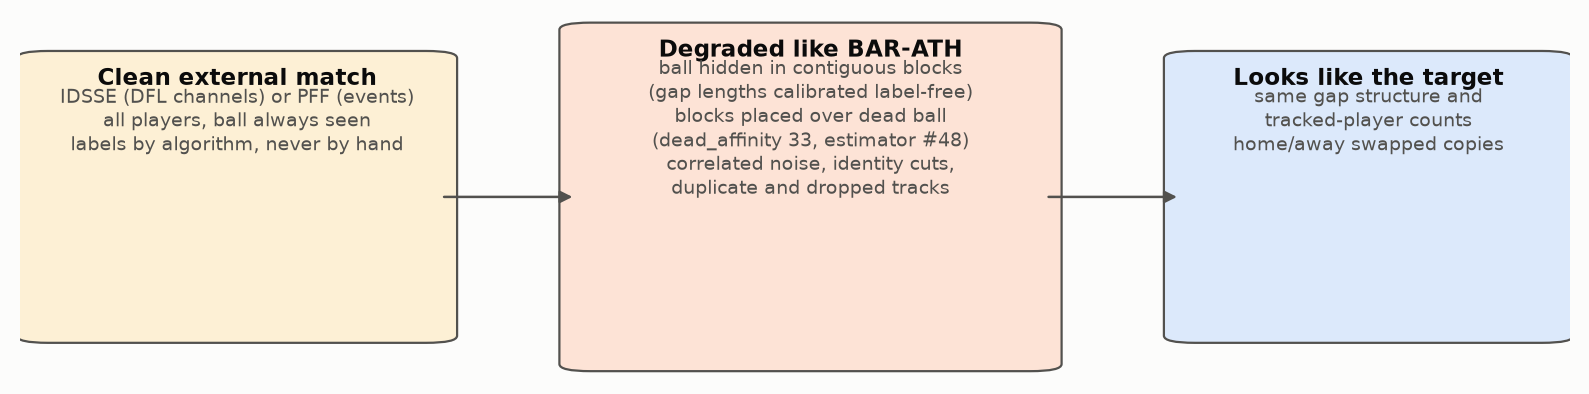
\includegraphics[width=0.95\linewidth]{degradation.png}
\caption{Every external match is made to look like BAR-ATH before training.}\label{fig:degr}\end{figure}

\paragraph{Where the ball goes missing (Issue \#48).} If gaps were placed at random, 41\,\% of hidden-ball frames would be dead. We built a label-free estimator: ball-free player features, a classifier trained on other matches, and prior-shift EM per tracked-player stratum. It was validated on IDSSE with planted affinities and on PFF and Metrica. On BAR-ATH it finds that \textbf{at least about 80\,\%} of hidden-ball graded frames are dead. The tracker loses the ball mostly during stoppages: replays, close-ups, the ball out of play. The degrader now places gaps over dead ball with that affinity (\code{dead\_affinity} 33, realised odds ratio 12--19), and the models are trained in that world.
\fig{hidden_ball_world.png}{Left: dead share of hidden-ball frames under three views. Right: training in the estimated world, +0.017 on the primary criterion with every seed positive.}

\subsection{Specialists A and B}
The per-frame features cover:
\begin{itemize}
\item distances to the three nearest players of each team and their difference;
\item Link--Hoernig control weights [1] and a touch score;
\item dynamic goalkeepers, spectral and convex-hull team areas and their 2\,s derivatives;
\item velocity coherence $R=\lVert \frac{1}{N}\sum_i \mathbf{v}_i/\lVert\mathbf{v}_i\rVert \rVert$ and line advance;
\item ball memory: last and next seen position and possessor, and time since and until the ball was seen.
\end{itemize}
\textbf{Specialist A} (ball visible) and \textbf{Specialist B} (ball hidden: collective physics, coherence, memory, dead-ball cues, a soft Smart Tagging prior) are LightGBM classifiers [5]. They run with \code{deterministic=True}, one thread and seed 0, and are calibrated by out-of-fold temperature [6] on whole held-out matches. They are fused per frame by ball visibility into $\log p[N,3]$, rounded to $10^{-6}$. On other matches with the ball hidden, Specialist B finds the right team on 0.85 of alive frames, against 0.62 for ``last touch''.

\subsection{Sequence model (Issues \#72--\#73)}
A non-causal dilated TCN [3,4] reads the specialists' feature matrix:
\begin{itemize}
\item 8 residual blocks, dilations 1 to 128, 64 channels, receptive field about $\pm$20\,s, 0.2\,M parameters;
\item an H/A/D head and a turnover head;
\item trained on degraded IDSSE (both worlds) and PFF matches 20--55, which are never in an evaluation cell;
\item two training seeds, averaged.
\end{itemize}
The weights are exported to \code{.npz} and run in \textbf{NumPy} (parity with PyTorch to $10^{-6}$), so the submission needs no PyTorch. The TCN is mixed into the emissions in log space:
\begin{equation}
\log p_t = (1-w_t)\,\log p^{\mathrm{spec}}_t + w_t\, s\, \log p^{\mathrm{TCN}}_t,\qquad
w_t=\begin{cases}1.0 & \text{ball hidden}\\ 0.5 & \text{ball visible}\end{cases},\quad s=0.8.
\end{equation}
The visible-ball weight and the scale were chosen from a \textbf{preregistered grid of five} (Figure~\ref{fig:grid}), posted before any score was seen. The winner beats the reference by +0.057 on the primary criterion, and every seed and both guards improve.
\begin{figure}[H]\centering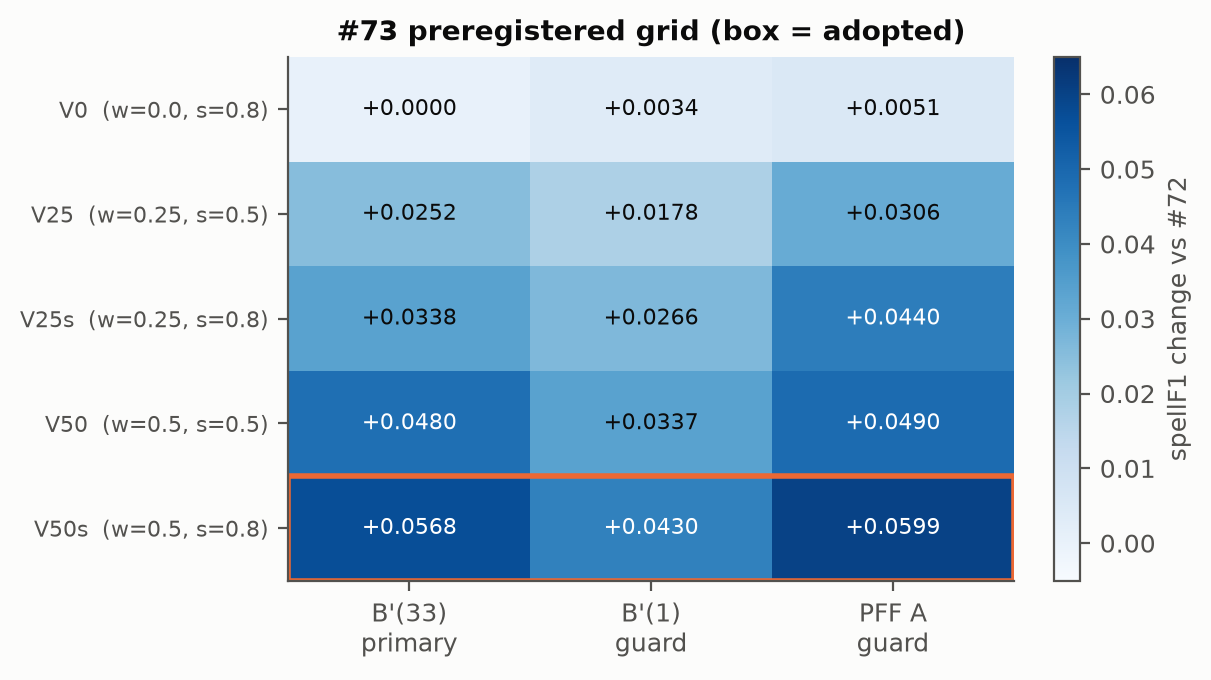
\includegraphics[width=0.62\linewidth]{grid73.png}
\caption{\#73 grid: spellF1 change against the \#72 reference on the primary criterion and both guards.}\label{fig:grid}\end{figure}

\subsection{Decoding for the metric}
Each graded half is decoded on its own by a Viterbi [7] with \textbf{time-dependent} transitions (Figure~\ref{fig:dec}):
\begin{equation}
\hat y = \operatorname*{arg\,max}_{y_{1:T}} \sum_t \Big[\log p_t(y_t) + \log A_t(y_{t-1}, y_t)\Big].
\end{equation}
\begin{itemize}
\item $\log A_t(H,A)$ is $-11.5$ at rest and opens to $-1.4$ within $\pm$5 frames of a touch by the gaining team (or, moderately, inside a long ball gap).
\item $H/A\to D$ opens with dead-ball evidence. $D\to$\,team stays closed until the evidence drops or a restart frame $t^*$ is reached.
\item The kernel is compiled with numba and has a bit-identical NumPy fallback; the decode takes under 0.2\,s.
\end{itemize}
\begin{figure}[H]\centering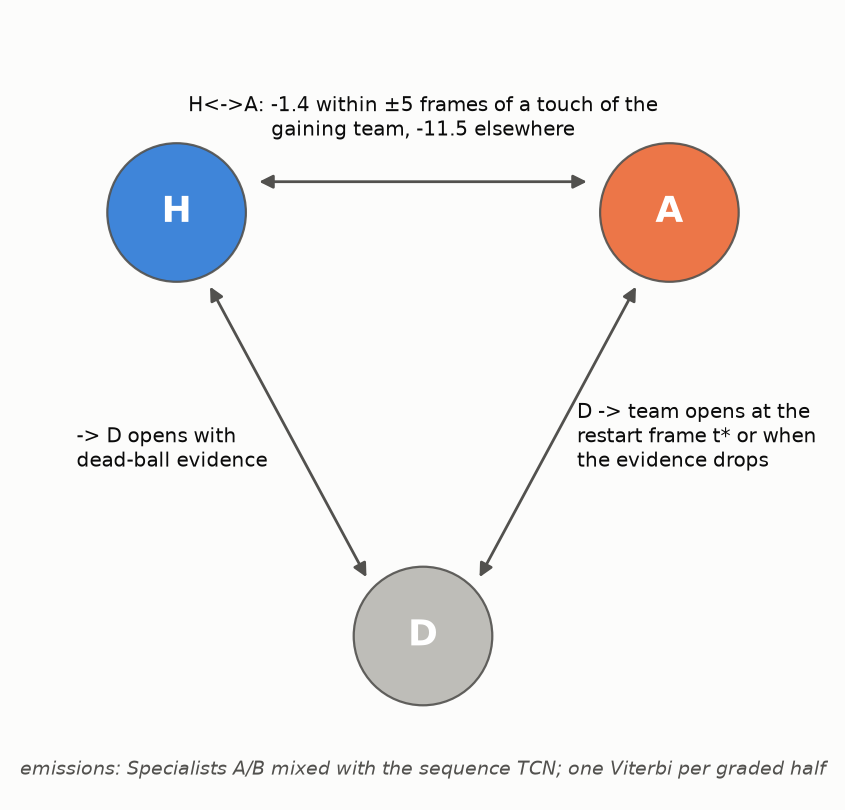
\includegraphics[width=0.4\linewidth]{decoder_states.png}
\caption{Decoder states and when each transition opens.}\label{fig:dec}\end{figure}
A \textbf{spell optimiser} then cleans the result:
\begin{itemize}
\item it absorbs H$\to$A$\to$H micro-possessions shorter than about 1\,s (0.98\,s, tuned on other matches), unless the ball is visible and shows a double touch;
\item it bridges long possessions with a \code{D} over $\geq$\,4\,s dead-evidence valleys that coincide with a touchline or set piece;
\item the \textbf{contract} writes \code{X} outside the graded blocks, \code{D} in the second-half pre-kick-off interval and no internal \code{X}, and validates the file with the official \code{validate\_submission.py}.
\end{itemize}

\section{The possession rules we implement}
\fig{possession_rules.png}{From touches to possession: a failed challenge, a controlled regain, a stoppage and a restart.}
\begin{table}[H]\centering\small
\begin{tabularx}{\linewidth}{>{\bfseries}p{3.4cm}L}
\toprule
\normalfont situation & rule\\
\midrule
Possession & from the touch that wins the ball until the other team's winning touch\\
Loose balls, balls in flight & the state is held: the last team in control keeps the ball until the other team touches it\\
Challenges and duels & a change needs a touch by the gaining team; simultaneous contact does not flip by itself; flickers $<$\,1\,s are absorbed unless the ball is visible with a double touch\\
Ball out of play, fouls, goals & \code{D} from the evidence of the stoppage until the restart frame $t^*$ found in the tracking; a \code{D} always splits a possession\\
Restarts & the team taking the restart, from the moment the ball leaves rest; unresolved throw-ins keep both \code{D}$\to$\code{H} and \code{D}$\to$\code{A} open\\
Hidden ball & the last and next possessor are carried over the gap with decaying confidence; in long gaps the change lands where the collective movement reverses\\
Ungraded frames & \code{X} outside the graded blocks (from \code{games.py}), never inside; nothing crosses a half boundary\\
\bottomrule
\end{tabularx}
\end{table}

\section{How we decided: one rule, 31 experiments}
The public window cannot rank methods, so every idea went through the same protocol, written down before any measurement:
\begin{itemize}
\item it is built in its own branch and issue, with its own tests;
\item it is measured against the current default on B$'$(33) with evaluation seeds 0--2, with B$'$(1) and PFF~A as guards;
\item it is \textbf{adopted only if} the mean spellF1 gain is $\geq$\,+0.010 and no seed falls below $-0.003$;
\item otherwise the code stays, switched off by configuration.
\end{itemize}
Two correctness fixes (\#50, \#51) were adopted on their own merit.
\fig[0.8]{experiment_ledger.png}{Every idea and its measured effect. Adopted ideas are blue; the dashed line is the adoption bar.}
Among the ideas left off are several that are popular elsewhere:
\begin{itemize}
\item a CRF head ($-0.022$);
\item expected-spellF1 / minimum-Bayes-risk decoding (about 0);
\item semi-Markov durations ($-0.003$);
\item a larger TCN ensemble (+0.0097, just below the bar);
\item pseudo-labels on BAR-ATH ($-0.016$);
\item pre-trained and self-supervised ball detectors on the tactical video, within 0.3\,m in only about 15\,\% of frames where about 0.2\,m would be needed;
\item broadcast synchronisation, which fills only 7.4\,\% of hidden tactical-ball frames (+0.005).
\end{itemize}
We prefer a smaller, verified system to a larger one tuned on noise.

\section{Assets used, tried and dropped}
\begin{table}[H]\centering\small
\begin{tabularx}{\linewidth}{p{4.2cm}p{2.6cm}L}
\toprule
asset & status & how\\
\midrule
Tactical ATD and metadata XML & used & all geometry, kinematics and features; slot teams\\
Smart Tagging XML & used & set-piece and goal windows (search windows for $t^*$), throw-in teams, a weak phase prior\\
Tactical homography & loaded, checked & consumed only by the optional vision stages, which are off\\
Broadcast ATD + homography & tried, off & 63\,\% of blocks synchronised; the TV ball fills 7.4\,\% of hidden frames, +0.005\\
Tactical / broadcast video & tried, off & YOLO, multi-frame, pre-trained and self-supervised detectors measured label-free on the real video; no video is processed for the submission\\
Aerial-ball filter & built, off & lowered spellF1 on degraded external matches (touches at kicks and landings are real boundaries)\\
Public 5-minute ground truth & pipeline check only & alignment and format; never used to choose or tune\\
Official scorer, \code{games.py}, starter & used, unmodified & metric, graded blocks, format check\\
IDSSE, PFF, Metrica, SkillCorner & other matches only & see Section 4.3 and Appendix~A\\
\bottomrule
\end{tabularx}
\end{table}
No private ground truth, no human-produced data about the provided game, no hand labelling and no manual correction. Every label in the file comes out of the code in the repository.

\section{Limitations and what we would do next}
\begin{itemize}
\item \textbf{Missed turnovers.} The route predicts fewer possessions than the truth: 2228 against 2759 on the 8 unseen PFF matches. It misses 45\,\% of H$\leftrightarrow$A turnovers with the ball visible and 54\,\% with the ball hidden. Issue \#79 showed that when a turnover is missed, the emissions carry no trace of it. The limit is the information in the tracking, not the decoder.
\item \textbf{Player dropout} (14.2\,\% of frames with fewer than 20 players) has no counterpart in the external matches. 91\,\% of those frames lie inside ball gaps, so a high \code{D} share there is plausible but cannot be validated externally.
\item \textbf{Domain shift.} We know BAR-ATH's noise only through label-free aggregates. The two proxies (IDSSE and PFF) sometimes disagree on the size of a trade-off. Match-to-match noise on spellF1 is about 0.04. Smart Tagging weights cannot be tuned, because no external match has Smart Tagging.
\item \textbf{Next steps:} a ball detector trained for this tactical camera (we measured that it needs about 0.2\,m accuracy); labelled matches in Metrica's own tracking convention; a player-level set encoder in front of the TCN for the hidden-ball turnovers.
\end{itemize}

\section{Reproduction}
\begin{tcolorbox}[colback=black!85,colupper=white,boxrule=0pt,arc=2pt,left=6pt,right=6pt]
\footnotesize\ttfamily
python -m venv .venv \&\& .venv\textbackslash Scripts\textbackslash activate\\
pip install -r requirements.txt \&\& pip install -e . -{}-no-deps\\
\# unpack the organisers' bundle into data/ (tactical/ and broadcast/)\\
python scripts/generate\_submission.py -{}-data-dir data -{}-specialists load -{}-team "Opus Operandi"\\
python evaluation/validate\_submission.py "outputs/Opus Operandi.csv"\\
\# sha256 40f95b38fbcc942de6492a102ea74d72e180689e6f3b59c805d61edaa5116a7b
\end{tcolorbox}
\begin{itemize}
\item \textbf{Dependencies.} All are pinned (Python $\geq$\,3.10; developed on 3.13, CI on 3.11).
\item \textbf{Determinism.} \code{PYTHONHASHSEED=0}, fixed seeds, deterministic single-thread LightGBM, NumPy TCN inference, and every decoder input rounded to $10^{-6}$. Two runs give the same SHA256, and so do the numba and NumPy decoders.
\item \textbf{Committed models.} The submission uses only \code{models/specialists.json} and \code{models/sequence\_tcn.json}. \code{scripts/train\_specialists.py} and \code{scripts/train\_sequence.py} rebuild them from the external matches.
\item \textbf{CI.} Ruff, more than 500 tests, a data-leak gate, and two full-length synthetic runs whose SHA256 must match.
\item \textbf{Figures.} \code{python scripts/make\_figures.py} redraws every figure in this document.
\end{itemize}

\appendix
\section{Training and validation data: provenance}
\begin{table}[H]\centering\footnotesize
\begin{tabularx}{\linewidth}{p{2.4cm}LLp{3.6cm}}
\toprule
dataset & source and licence & who labelled it, and how & how much\\
\midrule
IDSSE / DFL Sportec open data & Bassek et al., \emph{Scientific Data} 12, 195, 2025 (\href{https://doi.org/10.1038/s41597-025-04505-y}{doi:10.1038/s41597-025-04505-y}); data \href{https://doi.org/10.6084/m9.figshare.28196177}{doi:10.6084/m9.figshare.28196177}, also Hugging Face \code{pysport/idsse-data}; CC BY 4.0 & DFL-provided ball-status and possession channels; our labels are derived mechanically from them, as the competition derives its ground truth from tracking channels & 7 Bundesliga matches at 25\,fps: J03WMX, J03WN1, J03WOH, J03WOY, J03WPY, J03WQQ, J03WR9\\
PFF FC World Cup 2022 open data & \url{https://data.pff.com}, free public access under PFF's terms, accepted by the team; not redistributed & PFF event data (\code{OTB} ball owner, \code{OUT} dead ball, set-piece restarts); labels derived by replaying the events & 64 converted: first 20 by name for the specialists (weight 0.5), matches 20--55 for the TCN, 8 never used (pff\_3852--pff\_3859)\\
Metrica Sports sample data & \url{https://github.com/metrica-sports/sample-data}; no licence file, used locally only & Metrica events: control events give possession, stoppages give \code{D} & Games 1--3; evaluation only\\
SkillCorner open data & \url{https://github.com/SkillCorner/opendata}, MIT & \code{phases\_of\_play} (gaps give \code{D}) & 20 A-League 2024/25 matches; dropped\\
\bottomrule
\end{tabularx}
\end{table}
The labelling rules are in \code{mtah2027-external-benchmarks/docs/LABELLING\_RULES.md}. No label, threshold or hyper-parameter comes from the provided game, and none of the data was labelled by our team by hand.

\section{Release, fallbacks and other commands}
\begin{table}[H]\centering\footnotesize
\begin{tabular}{lll}
\toprule
file & SHA256 & configuration\\
\midrule
\textbf{submitted} (\#73) & \texttt{\scriptsize 40f95b38fbcc942de6492a102ea74d72e180689e6f3b59c805d61edaa5116a7b} & default\\
fallback (\#72) & \texttt{\scriptsize a31c0a3c864fa6ce16bc39c1f3d3b51a45b9bd2abc1d2bfbbb6cc223b08b3a6a} & visible weight 0.0, scale 0.5\\
fallback (pre-\#72) & \texttt{\scriptsize cac8927c2adc1b1a6778d0045a2fae0ba4437aee8ea10a889de02db7552d0c7b} & sequence model off\\
\bottomrule
\end{tabular}
\end{table}
\begin{tcolorbox}[colback=black!85,colupper=white,boxrule=0pt,arc=2pt,left=6pt,right=6pt]
\scriptsize\ttfamily
python scripts/generate\_submission.py -{}-data-dir data -{}-specialists load -{}-kpi \ \ \# + KPI dashboard\\
python scripts/generate\_submission.py -{}-data-dir data -{}-model-variant mixed \ \ \# gap|mixed|calib|idsse|pff\\
python scripts/generate\_submission.py -{}-synthetic -{}-out /tmp/sub.csv \ \ \# self-check without data (CI)\\
python scripts/make\_figures.py \ \ \# redraws docs/figures/
\end{tcolorbox}

\section{Reference points on the degraded IDSSE matches}
\begin{table}[H]\centering\small
\begin{tabular}{lcc}
\toprule
route (first, uncalibrated degrader) & spellF1 & macroF1\\
\midrule
Official-style baseline (nearest player, majority vote) & 0.215 & 0.440\\
Heuristic route (last toucher, dead-ball score, decoder) & 0.435 & 0.773\\
Specialists, IDSSE only & 0.642 & 0.910\\
Specialists (Milestone 9 model), complete ball, no degradation & 0.750 & 0.948\\
\bottomrule
\end{tabular}
\end{table}

\begin{thebibliography}{10}\small
\bibitem{lh} D.~Link, M.~Hoernig. Individual ball possession in soccer. \emph{PLoS ONE} 12(7), 2017.
\bibitem{idsse} M.~Bassek, R.~Rein, H.~Weber, D.~Memmert. An integrated dataset of spatiotemporal and event data in elite soccer. \emph{Scientific Data} 12, 195, 2025.
\bibitem{bai} S.~Bai, J.~Z.~Kolter, V.~Koltun. An empirical evaluation of generic convolutional and recurrent networks for sequence modeling. arXiv:1803.01271, 2018.
\bibitem{lea} C.~Lea, M.~D.~Flynn, R.~Vidal, A.~Reiter, G.~D.~Hager. Temporal convolutional networks for action segmentation and detection. \emph{CVPR}, 2017.
\bibitem{lgbm} G.~Ke et al. LightGBM: a highly efficient gradient boosting decision tree. \emph{NeurIPS}, 2017.
\bibitem{guo} C.~Guo, G.~Pleiss, Y.~Sun, K.~Q.~Weinberger. On calibration of modern neural networks. \emph{ICML}, 2017.
\bibitem{viterbi} A.~Viterbi. Error bounds for convolutional codes and an asymptotically optimum decoding algorithm. \emph{IEEE Trans. Information Theory} 13(2), 1967.
\bibitem{sg} A.~Savitzky, M.~J.~E.~Golay. Smoothing and differentiation of data by simplified least squares procedures. \emph{Analytical Chemistry} 36(8), 1964.
\bibitem{asrf} Y.~Ishikawa, S.~Kasai, Y.~Aoki, H.~Kataoka. Alleviating over-segmentation errors by detecting action boundaries. \emph{WACV}, 2021.
\bibitem{data} PFF FC FIFA World Cup 2022 open data (data.pff.com); Metrica Sports sample data (github.com/metrica-sports/sample-data); SkillCorner open data (github.com/SkillCorner/opendata).
\end{thebibliography}

\end{document}
